\documentclass[12pt,a4paper]{article}

\usepackage[a4paper, total={5.7in, 9in}]{geometry}
\usepackage[T1]{fontenc}
\usepackage[utf8]{inputenc}
\usepackage{graphicx}
\IfFileExists{booktabs.sty}{%
    \usepackage{booktabs}%
}{%
    \newcommand{\toprule}{\hline}
    \newcommand{\midrule}{\hline}
    \newcommand{\bottomrule}{\hline}
}
\usepackage{xcolor}
\usepackage{amsmath}
\usepackage{listings}
\usepackage{float}
\usepackage{tabularx}
\setlength{\emergencystretch}{1.25em}
\setlength{\parindent}{0pt}
\setlength{\parskip}{0.55em}
\setlength{\leftmargini}{1.4em}
\setlength{\labelsep}{0.45em}
\renewcommand{\labelitemi}{\textbullet}
\makeatletter
\AtBeginDocument{%
    \def\@listi{%
        \leftmargin\leftmargini
        \rightskip 0pt plus 1fil
        \topsep 0.35em
        \parsep 0pt
        \itemsep 0.3em
        \partopsep 0pt
    }%
    \let\@listI\@listi
}
\makeatother
\let\originalitemize\itemize
\renewcommand{\itemize}{\originalitemize\rightskip 0pt plus 1fil\relax}

\lstdefinestyle{nutrimas}{
    basicstyle=\ttfamily\footnotesize,
    frame=single,
    rulecolor=\color{black!20},
    backgroundcolor=\color{black!3},
    breaklines=true,
    columns=fullflexible,
    keepspaces=true,
    showstringspaces=false,
    aboveskip=0.8em,
    belowskip=0.8em
}
\lstset{style=nutrimas}
\renewcommand{\abstractname}{Abstract}
\renewcommand{\contentsname}{Contents}
\renewcommand{\figurename}{Figure}
\renewcommand{\tablename}{Table}
\renewcommand{\lstlistingname}{Code}
\renewcommand{\refname}{References}

\usepackage{tikz}
\usetikzlibrary{shapes.geometric, arrows.meta, positioning, fit, calc}
\usepackage{hyperref}
\hypersetup{
    colorlinks=true,
    linkcolor=blue!45!black,
    citecolor=blue!45!black,
    urlcolor=blue!55!black
}

\begin{document}
\title{Nutri-MAS: a hybrid multi-agent system for personalized nutritional assistance}
\author{Acossi Giorgio Roberto - S5339095\\
{\em acossigiorgio@gmail.com}}
\date{July 2026}
\maketitle

\begin{center}
\textbf{Project source code:}
\href{https://github.com/acossi-giorgio/nutri-mas}{\texttt{github.com/acossi-giorgio/nutri-mas}}
\end{center}

\section{Details of the proposal}
\label{sec:yourProposal}

\subsection{Proposal specification}
\label{subsec:specification}

Nutri-MAS is a conversational assistant that combines reactive agents, BDI agents, and LLM-based agents. 
The system collects the user's profile, calculates indicative caloric targets, builds a weekly plan, 
generates recipes, records the meals actually consumed, and rebalances the subsequent slots when the plan is modified. 

\subsection{Type of proposal}
\label{subsec:kind}
Type of proposal is creative. The main objective is to experiment with how agents with different decision-making models can
collaborate in the same system. 
\emph{Nutri-MAS} combines three types of agents:
\begin{itemize}
    \item \textbf{BDI agents}: they manage logic based on beliefs and rules, such as planning.
    \item \textbf{LLM agents}: they manage linguistic understanding and textual creativity.
    \item \textbf{Reactive agents}: they manage direct interaction with the user.
\end{itemize}

\subsection{Difficulty level of the proposal}
\label{subsec:points}
The proposed difficulty level depends greatly on the complexity of the implementation.
The complexity of the project does not depend only on the number and quality of the functionalities
implemented, but above all on the integration of heterogeneous agents within
a single operational flow. The system must translate requests expressed in
natural language into structured commands and orchestrate the
collaboration between BDI agents and LLM-based agents, characterized by different
decision-making models and reasoning capabilities.

Some simplifications of the domain have been adopted to make the
more complex aspects of meal planning manageable. These choices reduce
the breadth of the problem, but they do not eliminate the main difficulty, represented
by the end-to-end functional integration of the different components of the system.
The difficulty of the project has been proposed as \emph{medium-hard}.

\section{Introduction}
\label{sec:intro}

\emph{Nutri-MAS} is a hybrid multi-agent system for personalized nutritional
assistance, meal planning, and recipe generation. This
domain requires coordinating different needs: respecting the caloric,
dietary, and temporal constraints of the individual user, proposing sufficiently
varied recipes, and reacting to deviations from the plan. If, for example, the user consumes a
meal different from the one expected, the system must record the event and
redistribute the residual budget over the subsequent slots.

Nutri-MAS assigns to BDI agents the logic based on
beliefs and rules, such as planning and monitoring; to LLM agents it entrusts
linguistic understanding and recipe generation; a reactive agent finally manages
access to the system. Through the conversational interface the user
can create their own profile, generate and consult a weekly plan,
also record off-plan meals, and check the residual caloric budget.

\subsection{High-level architecture}

\begin{figure}[H]
\centering
\resizebox{0.9\textwidth}{!}{%
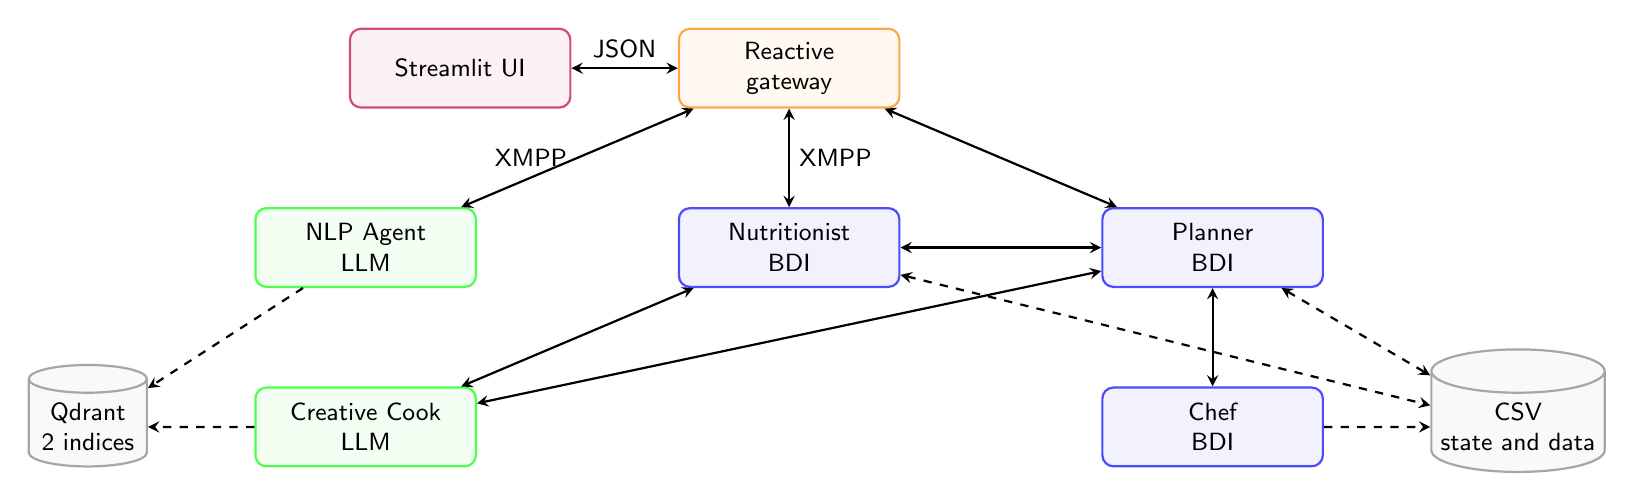
\begin{tikzpicture}[
  >=stealth,
  node distance=1.25cm and 1.35cm,
  every node/.style={font=\sffamily\small},
  bdi/.style={rectangle, draw=blue!70, fill=blue!5, rounded corners, minimum width=2.8cm, minimum height=1cm, align=center, thick},
  llm/.style={rectangle, draw=green!70, fill=green!5, rounded corners, minimum width=2.8cm, minimum height=1cm, align=center, thick},
  react/.style={rectangle, draw=orange!70, fill=orange!5, rounded corners, minimum width=2.8cm, minimum height=1cm, align=center, thick},
  ui/.style={rectangle, draw=purple!70, fill=purple!5, rounded corners, minimum width=2.8cm, minimum height=1cm, align=center, thick},
  db/.style={cylinder, draw=gray!70, fill=gray!5, shape border rotate=90, aspect=0.25, align=center, minimum height=1.2cm, minimum width=1.5cm, thick}
]

\node[ui] (streamlit) {Streamlit UI};
\node[react, right=of streamlit] (gateway) {Reactive\\gateway};

\node[llm, below left=of gateway, xshift=-1.2cm] (nlp) {NLP Agent\\LLM};
\node[bdi, below=of gateway] (nutri) {Nutritionist\\BDI};
\node[bdi, below right=of gateway, xshift=1.2cm] (planner) {Planner\\BDI};
\node[bdi, below=of planner] (chef) {Chef\\BDI};
\node[llm, below=of nlp] (cook) {Creative Cook\\LLM};

\node[db, left=of cook] (qdrant) {Qdrant\\2 indices};
\node[db, right=of chef] (csv) {CSV\\state and data};

\draw[<->, thick] (streamlit) -- node[above] {JSON} (gateway);
\draw[<->, thick] (gateway) -- node[left] {XMPP} (nlp);
\draw[<->, thick] (gateway) -- node[right] {XMPP} (nutri);
\draw[<->, thick] (gateway) -- (planner);
\draw[<->, thick] (nutri) -- (planner);
\draw[<->, thick] (planner) -- (chef);
\draw[<->, thick] (planner) -- (cook);
\draw[<->, thick] (nutri) -- (cook);
\draw[->, dashed, thick] (nlp) -- (qdrant);
\draw[->, dashed, thick] (cook) -- (qdrant);
\draw[<->, dashed, thick] (nutri) -- (csv);
\draw[<->, dashed, thick] (planner) -- (csv);
\draw[->, dashed, thick] (chef) -- (csv);

\end{tikzpicture}%
}
\caption{High-level architecture of Nutri-MAS}
\end{figure}

The architecture of Nutri-MAS is composed of a conversational UI, a Gateway, and a set of specialized agents.
The UI communicates with the Gateway by means of JSON messages. The Gateway connects the UI to the multi-agent system, 
validates the messages, and controls their routing.

The multi-agent system adopts a hybrid architecture composed of three BDI agents and two LLM-based agents. 
The BDI agents handle the system’s state and enforce its rules: the Nutritionist manages the user profile, 
nutritional targets, and dietary logs; the Planner constructs the weekly meal plan; and the Chef selects 
food templates that satisfy the specified constraints. The LLM-based agents complement these functions: 
the NLP Agent translates natural-language requests into structured commands, while the Creative Cook turns 
the templates and constraints provided by the BDI agents into complete recipes.

Communication between the agents takes place through XMPP, while the content of the application messages uses a representation
compatible with the AgentSpeak syntax. State persistence is entrusted to CSV files that contain the user profile and the meal plans. Qdrant supports the semantic search of the linguistic examples of the NLP Agent and
of the ingredients used by the Creative Cook.

\section{Technological stack}

The system was developed using Python as the programming language and the SPADE, SPADE-BDI and SPADE-LLM libraries for agent management, 
Streamlit for the UI, Qdrant for semantic search and LiteLLM as a proxy for access to Large Language Models.

\subsection{Streamlit}

The UI was implemented with the Python library Streamlit. Communication between the UI
and the Gateway takes place through two queues, one carries the user's
messages toward the system, while the other transfers to the UI the responses
and events produced by the agents.

The interface keeps message input available even during
agent processing. The questions and answers generated by the system preserve an
explicit context, used by the NLP Agent to associate the user's response
with the correct AgentSpeak command.

\subsection{SPADE}

SPADE (Smart Python Agent Development Environment) is a Python framework for
the development of distributed multi-agent systems. The framework provides the
basic functionalities to define reactive agents, manage their life cycle and
allow message exchange through the XMPP protocol. 
The behaviour of each agent is defined and organized through
behaviours. To these functionalities are added the SPADE-BDI and SPADE-LLM extensions.

SPADE-BDI introduces a deliberative model based on beliefs, desires and
intentions, in which the behaviour of agents is defined through
AgentSpeak rules and plans. 

SPADE-LLM makes it possible to integrate Large Language Models within agents,
defining their behaviour through instructions and context and allowing them
to use tools to access application
functionalities and interact with the other components of the system.

\subsection{XMPP}

XMPP (Extensible Messaging and Presence Protocol) is an IETF standard for the
near-real-time exchange of structured data through XML streams. The
protocol defines mechanisms for addressing, authentication and
message delivery, identifying each entity through an ID. 
In Nutri-MAS, each agent possesses a local ID used as
identity and communication address. SPADE manages the connection to the
XMPP server and the exchange of messages among agents, while the application
content of the messages is represented through commands in AgentSpeak syntax.

\subsection{SPADE-BDI}

The deliberative layer of Nutri-MAS is implemented through SPADE-BDI,
an extension that allows the execution of AgentSpeak programs within
SPADE agents. The Nutritionist, Planner and Chef agents extend
\texttt{BDIAgent} and load their respective AgentSpeak programs. In this
model, \emph{beliefs} represent the information that the agent considers
true, \emph{goals} describe the states that it intends to achieve and plans
specify how to react to events. Each plan in fact defines a triggering
event, a context that determines its applicability and a set of actions
to execute.

Custom Python actions constitute the link between
declarative reasoning and application functionalities, such as numerical
calculations, access to CSV files, data serialization and the exchange of
messages with non-BDI agents. This separation keeps decision-making
policies explicit in the AgentSpeak programs, entrusting Python with computational
and infrastructural operations.

\subsection{SPADE-LLM}

SPADE-LLM extends the SPADE agent model by introducing functionalities
based on Large Language Models. An LLM agent is configured through a
provider, a set of initial instructions (\emph{system prompt}) and a series
of tools.

The \emph{tools} are implemented as Python functions and described through a
schema that specifies their parameters and methods of use. The model can
select the necessary tools, provide the corresponding arguments and use
the obtained results to continue processing. A single request can
therefore involve multiple interactions between the model and the tools, up to the production
of the final result or the reaching of the configured limit.

\subsection{LiteLLM Proxy}

LiteLLM provides a uniform abstraction layer for access to different
LLM providers. In the project it is used as a proxy to expose both the APIs for
LLM text generation and those for the production of embeddings.
The model used was gpt-5.4 and text-embedding-3-large respectively for text generation and embedding.

\subsection{Qdrant}

Qdrant is a vector database designed to store embeddings and
retrieve contents based on their semantic similarity. Compared to a
search based on exact word matching, it makes it possible to identify
conceptually close elements even when they are described with
different expressions. Nutri-MAS uses it to support the semantic searches of the NLP
Agent and the Creative Cook.

\section{Data management}

Nutri-MAS uses two complementary forms of data management: CSV files,
used for persistence and for static datasets, and Qdrant collections,
used for semantic search.

\subsection{CSV data}

To provide the agents with a static knowledge base and preserve the
user's information across different executions of the application, Nutri-MAS
uses a persistence system based on CSV files. This solution was
preferred to a traditional database in order to reduce infrastructural
complexity.

The CSV files are divided into two main categories: persistent files, read
and updated during execution, and static datasets, used by the agents
in read-only mode. Overall, they perform three functions:

\begin{itemize}
    \item \textbf{Persistence}: preserves the user's state and history across successive executions.
    \item \textbf{Materialization}: stores the results produced by the planning process.
    \item \textbf{Static knowledge}: provides the agents with food templates,
    nutritional rules, and ingredient data.
\end{itemize}

During system startup, each agent loads or indexes the data under its responsibility. The
operational and control state of the BDI agents is represented by beliefs. Static reasoning
facts, including slot order, slot weights, schedules and slot compatibility, are declared in
the AgentSpeak programs; Python actions read those beliefs when they need the same information.
The Python code performs adaptation, calculation and persistence functions.
Persistent data are written back to the files when the systemis shut down.

\begin{table}[H]
\centering
\small
\setlength{\tabcolsep}{5pt}
\renewcommand{\arraystretch}{1.15}

\begin{tabularx}{\textwidth}{
    @{}
    p{0.21\textwidth}
    p{0.18\textwidth}
    X
    @{}
}
\toprule
File & Main agent & Description and use \\
\midrule

\texttt{user.csv}
& Nutritionist
& Contains the user's profile, including anthropometric data, activity
level, goals, allergens, diet type, and nutritional
targets. \\

\texttt{weight\_log.csv}
& Nutritionist
& Stores the weight history. \\

\texttt{meal\_log.csv}
& Nutritionist
& Records planned and actually consumed meals, together with calories,
macronutrients, and registration status. \\

\texttt{week\_plan.csv}
& Planner
& Contains the complete weekly plan, with recipes, ingredients, instructions,
and nutritional values. \\

\texttt{week\_plan\_}\newline
\texttt{template.csv}
& Planner
& Stores the selected abstract templates of the active plan, including their
target calories, macronutrients, and food categories. \\

\texttt{templates.csv}
& Chef
& Contains the candidate food templates, classified by slot, category,
and nutritional values. \\

\texttt{nutrition\_}\newline
\texttt{rules.csv}
& Planner
& Defines the variety and frequency constraints associated with food
categories, diet types, and slots of the weekly plan. \\

\texttt{ingredients.csv}
& Creative Cook
& Contains the ingredients and their nutritional values per 100 grams.
The dataset is semantically indexed to generate recipes and estimate
freely described meals. \\

\bottomrule
\end{tabularx}

\caption{Persistent data and reference datasets used by the agents}
\end{table}

\subsection{Qdrant collections}

The vector collections are built at startup from the data and
templates available in the project. During execution they are queried by the
agents to retrieve the elements semantically closest to their requests.

\begin{table}[H]
\centering
\small
\setlength{\tabcolsep}{5pt}
\begin{tabular}{@{}p{0.22\linewidth}p{0.20\linewidth}p{0.50\linewidth}@{}}
\toprule
Collection & Main agent & Description and use \\
\midrule

\texttt{ingredients}
& Creative Cook
& Semantically indexes the names of the ingredients coming
from the Australian Food Composition Database \cite{FSANZAFCDRelease3}. Each ingredient is associated with
its calorie, protein, carbohydrate, and fat values. \\

\texttt{nlp\_translations}
 & NLP Agent
 & Contains linguistic templates associated with the application messages available in the
 system. Through semantic search, the NLP Agent identifies the messages most
 suitable for the user's request and retrieves their structure from the registry. \\

\bottomrule
\end{tabular}
\caption{Vector collections used by Nutri-MAS}
\end{table}
The embeddings are generated through the embedding model configured in LiteLLM.

\section{Design and implementation of the agents}
\sloppy

The following table summarizes the main application functionalities associated with each agent.

\begin{table}[H]
\centering
\begin{tabular}{p{0.18\linewidth}p{0.70\linewidth}}
\toprule
Agent & Offered functionalities \\
\midrule
Gateway
& Integration between the UI and the MAS, including forwarding requests to the NLP Agent for translation, validating commands, and routing them \\

NLP
& Translation of requests in natural language into valid
application actions and conversion from AgentSpeak commands to responses in natural language. \\

Nutritionist
& Onboarding, target calculation, weight and meal logging, reminders,
recaps and rebalancing of nutritional plans. \\

Planner
& Generation of the nutritional plan, control of variety and frequencies,
plan consultation and local replanning of future meals. \\

Chef
& Selection of food templates compatible with diet, slot, calories,
macronutrients and constraints. \\

Creative Cook
& Generation of concrete recipes and nutritional estimation of meals described
freely. \\

\bottomrule
\end{tabular}
\caption{Map between agents and application functionalities}
\end{table}


\subsection{SPADE behaviours and execution model}

\subsection{Gateway Agent}

The Gateway connects the user interface to the multi-agent system and manages communication in
both directions. It sends messages in natural language to the NLP, which translates them into
AgentSpeak/Prolog commands; the Gateway then validates and forwards those commands to the recipient
agents. In the reverse path, it deterministically converts the technical responses of the agents
into validated UI events. It does not make nutritional decisions, but deals only with message
flow, validation and presentation.


Its operation is based on two cyclic behaviours. \texttt{LocalCommandBehaviour} retrieves from the
UI queue the user's messages and sends them to the NLP for translation; \texttt{GatewayBehaviour}
receives XMPP messages, forwards translated commands returned by the NLP to the domain agents and
publishes domain responses in the UI through the deterministic response renderer.

\subsection{NLP Agent}

The NLP Agent manages the translation between the natural language of the chat and the
AgentSpeak/Prolog commands accepted by the system. User requests are interpreted by an
\texttt{LLMAgent}; deterministic rendering of BDI responses is instead invoked by the Gateway and
does not require a second LLM translation.

The Gateway sends to the NLP Agent one of the following two formats:

\begin{lstlisting}[caption={Input formats of the NLP Agent}]
username: <name>
message: <user text>

username: <name>
question: <question shown to the user>
answer: <user reply>
\end{lstlisting}

The first format represents an autonomous request, for example ``Show me today's meal plan''.
The second is used when the user replies to a previous question. The Gateway includes
explicitly both the displayed question and the new answer, making it possible to interpret the
user's replies in the best way, which otherwise may be ambiguous.

A \emph{message} represents an operation that the user can request through the
chat. Its definition contains an identifier, a description, the recipient agent,
the SPADE performative and the schema needed to build the AgentSpeak performative.
All messages are saved in a JSON list, which constitutes the message registry.

Qdrant instead contains short linguistic templates used exclusively for retrieval. Each chunk
associates a possible user formulation with the identifier of a message:

\begin{lstlisting}[language=Python,caption={Example of indexed linguistic chunk}]
{
    "nl_template": "I ate {actual_food} for {meal_type}.",
    "message": "nutritionist.log_meal"
}
\end{lstlisting}

Several chunks can point to the same identifier, making it possible to represent different
formulations without duplicating the command definition. The search retrieves the semantically closest
points, removes duplicate identifiers and returns a number of candidates chosen by the model. 
The content of the template therefore influences only the initial selection.

For each retrieved identifier, the message registry provides the complete definition.
\begin{lstlisting}[language=Python,caption={Example of message definition in the registry}]
{
    "id": "nutritionist.get_daily_recap",
    "agent": "nutritionist",
    "message_performative": "achieve",
    "description": "Show today's calorie recap.",
    "signature": "get_daily_recap(Username)",
    "schema": {
        "functor": "get_daily_recap",
        "arity": 1,
        "type": "object",
        "properties": {
            "Username": {
                "type": "string"
            }
        },
        "required": ["Username"]
    }
}
\end{lstlisting}

The description helps the model distinguish semantically close operations, while signature and
schema establish structure, order, types and allowed values. The model therefore must not reconstruct
the command from the linguistic chunk, but only from the data of the registry.

The tools available for translation are:

\begin{itemize}
    \item \texttt{search\_message\_templates}: searches in Qdrant for templates semantically similar to 
    the request and returns the distinct identifiers of the candidate messages. The order of the results 
    indicates only the degree of similarity.
    \item \texttt{get\_message}: retrieves from the registry the definitions of the candidate messages, 
    including description, recipient, performative, signature and argument schema.
    \item \texttt{submit\_translation}: validates the ASL syntax, the arity, the absence of free variables and the 
    consistency between command and registered route, then transmits the result to the Gateway.
\end{itemize}

The translation process follows the following steps:

\begin{itemize}
    \item \textbf{Search}: the model performs semantic search to identify the candidate messages.
    \item \textbf{Selection}: it retrieves the corresponding definitions from the registry and selects the one consistent with the request.
    \item \textbf{Translation}: it fills the arguments with the data provided by the user and invokes
    \texttt{submit\_translation}, which validates and transmits the result to the Gateway.
\end{itemize}

The system prompt describes the translation workflow and the ways of using the tools,
without directly including the list of supported messages.
The latter are defined in the registry and associated with the linguistic templates indexed in Qdrant.
This separation makes the system extensible; in fact, it is possible to add new messages
without modifying the system prompt, keeping the general logic of the NLP Agent unchanged.

\subsection{Nutritionist Agent}

The Nutritionist manages the nutritional state of the user and coordinates the daily cycle of the
system. It maintains profile, objectives and logs, starts planning and reacts to events
that require confirmations or modifications of the plan. The decision rules are expressed by means of
BDI plans.

The beliefs of the Nutritionist represent the user's profile and nutritional objectives,
together with the history of meals, weight and the state of the operations in progress. The agent uses them
to adapt targets, monitor consumption and decide when to update or rebalance the plan.

The main BDI plans implement the following functionalities:
\begin{itemize}
    \item \textbf{Onboarding and profile management}: \texttt{check\_user\_profile} restores an existing profile or starts the collection of personal data, allergens, diet and culinary preferences. Profile-update plans persist changes and, when necessary, regenerate the weekly plan. In particular, a weight variation of at least 1\% causes calories and macronutrients to be recalculated, while reaching the target changes the objective to maintenance. The nutritional calculations are performed by Python actions invoked by these plans.
    \item \textbf{Daily monitoring}: reminder plans react to the \texttt{clock\_tick} produced by a \texttt{CyclicBehaviour} and request confirmation when a meal-slot time is crossed. Meal-tracking plans then confirm the planned recipe or ask the Creative Cook to estimate a different meal, updating the corresponding log beliefs.
    \item \textbf{Rebalancing}: after a deviation from the plan, \texttt{request\_rebalance\_after} calculates the residual nutritional budget and coordinates the Planner, Chef and Creative Cook to replace only subsequent meals. The beliefs \texttt{pending\_rebalances} and \texttt{pending\_rebalance\_origin} preserve the workflow state until all responses have arrived.
    \item \textbf{Consultation}: \texttt{get\_daily\_recap}, \texttt{get\_meal\_logs} and \texttt{get\_weight\_logs} read the current beliefs and use serialization actions to build the structured data returned to the Gateway.
\end{itemize}


\subsection{Planner Agent}

The Planner transforms the user's nutritional requirement into a weekly plan. It coordinates the
construction of the plan, keeps the progress state and waits for the responses of Chef and Creative
Cook before proceeding. The planning and control rules are expressed by means of BDI plans.

The beliefs of the Planner represent the received targets, the plan already built, the constraints of
variety and the progress state of the planning. The agent consults and updates them to
coordinate the choice of meals and avoid repetitions.

The main BDI plans implement the following functionalities:
\begin{itemize}
    \item \textbf{Weekly plan construction}: \texttt{build\_week\_plan} stores the user context and prevents concurrent generations. The Planner derives nutritional targets for the five slot types, obtains compatible template domains from the Chef and builds an assignment over the 35 weekly positions, enforcing daily variety and weekly category constraints. Python actions support the nutritional calculations and feasibility checks, while the BDI plans control the sequence of choices.
    \item \textbf{Recipe generation and plan activation}: once the template assignment is complete, the Planner asks the Creative Cook to produce each concrete recipe and stores the responses in \texttt{draft\_recipe\_row}. Only a complete draft is promoted to \texttt{planned\_recipe\_row}; otherwise the draft is discarded and the previous active plan remains available.
    \item \textbf{Local replanning}: \texttt{rebalance\_slot} applies the target received from the Nutritionist and coordinates Chef and Creative Cook to rebuild a single meal.
    \item \textbf{Consultation}: \texttt{get\_plan} reads \texttt{planned\_recipe\_row} and serializes the complete weekly plan for the Gateway.
\end{itemize}

\subsection{Chef Agent}

The Chef selects food templates compatible with the constraints of the plan. It does not directly generate
the recipes, but narrows the space of alternatives considering diet, slot, category, calories,
macronutrients and nutritional constraints. The selection rules are expressed by means of BDI plans and rules.

The beliefs of the Chef represent the available food templates and the criteria with which to evaluate
their compatibility with respect to the current request. The agent uses them to filter the alternatives
according to diet, slot, category, calories, macronutrients and exclusions. For weekly generation it
returns the complete valid domain; for local replanning it returns one strict candidate or reports failure.

The main BDI plans implement the following functionalities:
\begin{itemize}
    \item \textbf{Template selection}: \texttt{template\_candidate} filters the templates stored in \texttt{template\_for\_plan} according to diet, meal slot, calories, macronutrients and exclusions. Guided requests can also impose a required category. Python actions check numerical tolerances and introduce variability only among candidates already accepted by the BDI rules.
    \item \textbf{Candidate-domain provision}: for each slot-type target received during weekly generation, the Chef returns every valid template and then signals completion of the domain transfer.
\end{itemize}

\subsection{Creative Cook Agent}

The Creative Cook deals with managing two distinct operations. During
planning it transforms an abstract template into a concrete recipe with name, ingredients,
grammages, instructions and macronutrients. During tracking, instead, it interprets a meal described
freely and estimates its composition and nutritional values, also producing the template to use for
the subsequent rebalancing.

The Creative Cook does not maintain a BDI belief base: it accesses the user's nutritional context,
the constraints and targets of the request and the nutritional data of the ingredients. It uses this
information to generate compatible recipes or estimate the composition of a free meal.

The Creative Cook receives one of the following two AgentSpeak messages:

\begin{lstlisting}[caption={Input formats of the Creative Cook Agent}]
prepare_plan_slot(Username, Day, MealType, Template, TargetCalories, TargetProtein, TargetCarbs, TargetFat)
evaluate_free_meal(Username, Date, MealType, MealName, UserCalories)
\end{lstlisting}

The first format is sent by the Planner and contains the selected template together with the targets
of the slot. The second comes from the Nutritionist when the user declares having consumed a
meal different from the planned one; \texttt{UserCalories} can contain a value declared by the user.
The signature of the message determines the workflow and the allowed terminal tool, preventing
recipe generation and consumption evaluation from being combined.

The available tools are:

\begin{itemize}
    \item \texttt{query\_user\_nutrition\_context}: requests from the Nutritionist, in read-only mode, diet, allergens, culinary preferences, objective, daily calories and meal distribution, the response is handled through a dedicated behaviour.
    \item \texttt{query\_ingredient\_db}: performs a semantic search in the Qdrant database of ingredients with nutritional values per 100 g.
    \item \texttt{submit\_prepared\_recipe}: builds a \texttt{recipe} message with ingredients and grammages, instructions, calories and macros, then sends it to the Planner.
    \item \texttt{submit\_evaluated\_free\_meal}: builds a \texttt{free\_meal\_evaluated} message with estimated calories, macros and template, then sends it to the Nutritionist.
\end{itemize}

The process of preparing a recipe follows the following steps:

\begin{itemize}
    \item \textbf{Interpretation}: the model interprets the template and retrieves the nutritional context, checking allergens and diet first and then culinary preferences.
    \item \textbf{Search}: it searches semantically for the necessary ingredients, covering the main groups of the recipe, and uses only ingredients returned by the database.
    \item \textbf{Calculation}: it assigns grammages, estimates calories and macros from the values per 100 g and performs the estimation of portions with respect to the targets.
    \item \textbf{Sending}: it invokes \texttt{submit\_prepared\_recipe} to send the recipe to the Planner.
\end{itemize}

The process of evaluating a free meal follows the following steps:

\begin{itemize}
    \item \textbf{Search}: the model searches in the database for the full name of the meal, verifying whether there is a correspondence with an already prepared food.
    \item \textbf{Decomposition}: if the result is not sufficient, it decomposes the dish into its main ingredients and searches for them separately.
    \item \textbf{Estimation}: it calculates portions, calories and macronutrients; if the user indicated the calories, it adapts the macros to the declared total.
    \item \textbf{Classification}: it chooses the template that best represents the consumed meal.
    \item \textbf{Sending}: it invokes \texttt{submit\_evaluated\_free\_meal} to send the evaluation to the Nutritionist.
\end{itemize}

The system prompt encodes both the routing and the hierarchy of constraints. Allergens are a strong
constraint, the diet must always be respected and culinary preferences are applied only
when compatible with safety, template, available ingredients and targets. If no specific
preferences are present, the model favors traditional Italian cuisine. The text of the
preferences is treated exclusively as recipe data and cannot modify tools,
workflow or output format.

Allergens are free text and are treated by the prompt as a strong constraint: in case of doubt
the model must avoid the ingredient and choose a safer alternative. The instructions of the
recipe remain brief and do not repeat doses or the list of ingredients, already transmitted separately.
These constraints entrusted to the model are useful precautions, but they are not equivalent to a
deterministic clinical validation. The limit of eight interactions also reduces the risk of search cycles.

\subsection{Communication between BDI agents and non-BDI agents}

All agents communicate by means of messages transported over XMPP. The difference therefore does not concern
the communication protocol, but the way in which each type of agent interprets the
received messages. The LLM agents process requests through the SPADE-LLM behaviours, which
coordinate the local context of the LLM with the tool calls.

When a normal SPADE agent, such as the Gateway or the Creative Cook, sends a message to a
BDI agent, \texttt{TellBridge} and \texttt{AchieveBridge} adapt the application protocol to
AgentSpeak events. Both analyze the ASL body of the message: \texttt{TellBridge} translates a
\texttt{tell} performative into the addition of a belief, while \texttt{AchieveBridge} translates an
\texttt{achieve} performative into an achievement goal.

Between two BDI agents, on the other hand, no bridge is necessary. The AgentSpeak action \texttt{.send}
provided by SPADE-BDI builds an XMPP message in the native format of the extension and the
recipient's \texttt{BDIBehaviour} converts it directly into the corresponding event. The bridges
therefore remain confined to the connection between BDI and non-BDI agents.

\sloppy

\section{Workflow}

\subsection{Onboarding and first planning}

At startup the Nutritionist checks whether a complete user profile exists. If it does, the stored
profile is restored and the user is welcomed back without automatically regenerating the plan. If it
does not, the Nutritionist collects all required profile data and preferences in a fixed sequence,
calculates the goal and daily requirement, and starts generation of the first weekly plan.

\begin{figure}[H]
\centering
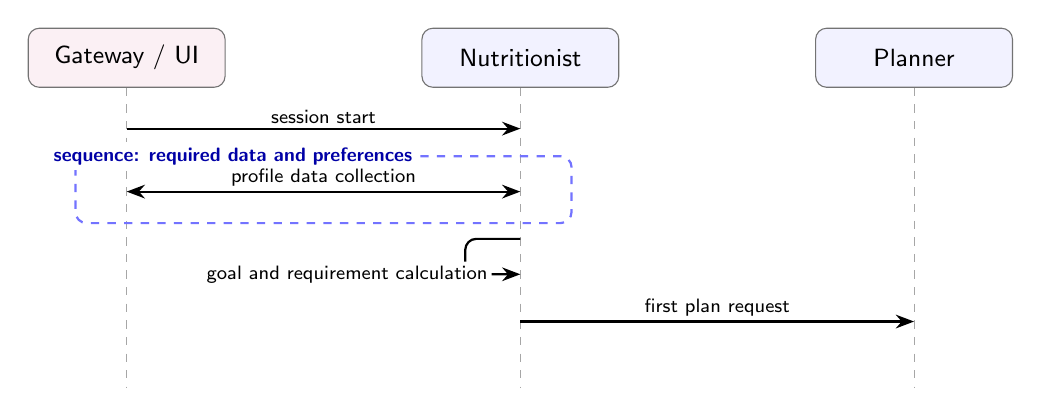
\begin{tikzpicture}[
    >=Stealth,
    actor/.style={rectangle, draw=black!55, rounded corners, fill=blue!5,
                  minimum width=2.5cm, minimum height=0.75cm, align=center,
                  font=\sffamily\small},
    message/.style={font=\sffamily\scriptsize, fill=white, inner sep=1.5pt}
]
\node[actor, fill=purple!6] (ui) at (0,0) {Gateway / UI};
\node[actor] (nutri) at (5,0) {Nutritionist};
\node[actor] (planner) at (10,0) {Planner};
\foreach \x in {ui,nutri,planner} {
    \draw[dashed, black!35] (\x.south) -- ++(0,-3.8);
}
\draw[->, thick] (0,-0.9) -- node[message, above]{session start} (5,-0.9);
\draw[rounded corners, thick, dashed, blue!55]
    (-0.65,-1.25) rectangle (5.65,-2.1);
\node[font=\sffamily\scriptsize\bfseries, text=blue!65!black,
      fill=white, inner sep=2pt] at (1.35,-1.25) {sequence: required data and preferences};
\draw[<->, thick] (0,-1.7) -- node[message, above]{profile data collection} (5,-1.7);
\draw[->, thick, rounded corners] (5,-2.3) -- ++(-0.7,0) -- ++(0,-0.45) --
    node[message, left]{goal and requirement calculation} (5,-2.75);
\draw[->, thick] (5,-3.35) -- node[message, above]{first plan request} (10,-3.35);
\end{tikzpicture}
\caption{UML diagram of the onboarding workflow}
\end{figure}

\subsection{Construction of the weekly plan}

The Nutritionist starts weekly generation after onboarding or an explicit regeneration request. The
Planner then coordinates construction of the weekly plan: it computes the nutritional targets and
requests from the Chef the complete domain of valid
templates for each of the five meal-slot types. The Chef filters its template
beliefs according to diet, slot, category, calorie and macronutrient constraints, returning
only strict candidates without introducing relaxed fallback templates when no
valid candidate is available.

The generation process is divided into two phases. During the first phase, the
candidate domains are stored as beliefs and a global AgentSpeak search is
performed over the 35 ordered meal slots of the week. Templates are assigned
while enforcing daily variety and weekly category-frequency constraints. Whenever a partial assignment becomes
infeasible, the relevant choices are reverted and an alternative candidate is
explored. This process produces a structured weekly template assignment.

During the second phase, each selected template is passed to the Creative Cook,
which turns it into a complete recipe by defining its ingredients, quantities,
and preparation instructions. The Planner temporarily stores the generated
recipes as beliefs and activates the draft only after all meal slots have been
materialized successfully. It then performs a staged replacement: the previous
active plan is cleared only when the complete draft is ready, after which the new
recipes and slot targets are promoted and transferred to the Nutritionist as beliefs.


\begin{figure}[H]
\centering
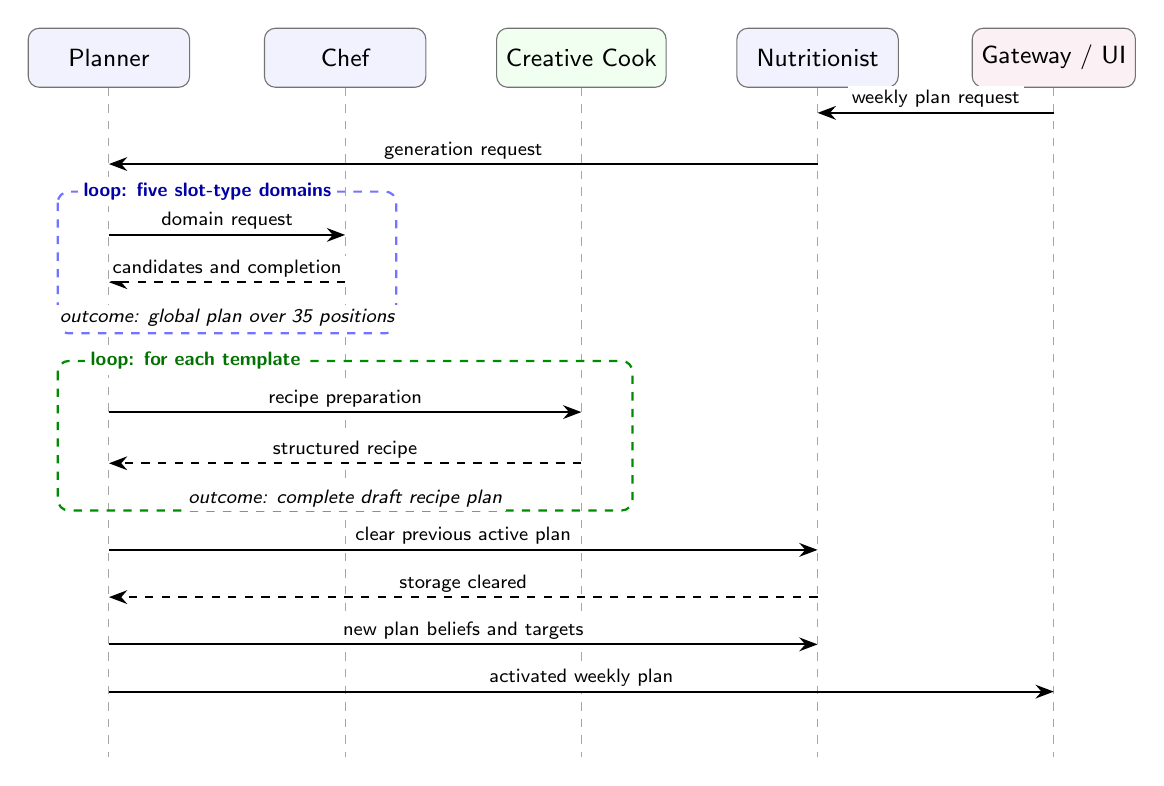
\begin{tikzpicture}[
    >=Stealth,
    actor/.style={rectangle, draw=black!55, rounded corners, fill=blue!5,
                  minimum width=2.05cm, minimum height=0.75cm, align=center,
                  font=\sffamily\small},
    message/.style={font=\sffamily\scriptsize, fill=white, inner sep=1.5pt}
]
\node[actor] (planner) at (0,0) {Planner};
\node[actor] (chef) at (3,0) {Chef};
\node[actor, fill=green!6] (cook) at (6,0) {Creative Cook};
\node[actor] (nutri) at (9,0) {Nutritionist};
\node[actor, fill=purple!6] (ui) at (12,0) {Gateway / UI};
\foreach \x in {planner,chef,cook,nutri,ui} {
    \draw[dashed, black!35] (\x.south) -- ++(0,-8.5);
}

\draw[->, thick] (12,-0.7) -- node[message, above]{weekly plan request} (9,-0.7);
\draw[->, thick] (9,-1.35) -- node[message, above]{generation request} (0,-1.35);

% First phase: domain collection and global AgentSpeak search.
\draw[rounded corners, thick, dashed, blue!55]
    (-0.65,-1.7) rectangle (3.65,-3.5);
\node[font=\sffamily\scriptsize\bfseries, text=blue!65!black,
      fill=white, inner sep=2pt] at (1.25,-1.7) {loop: five slot-type domains};
\draw[->, thick] (0,-2.25) -- node[message, above]{domain request} (3,-2.25);
\draw[->, thick, dashed] (3,-2.85) -- node[message, above]{candidates and completion} (0,-2.85);
\node[message, font=\sffamily\scriptsize\itshape] at (1.5,-3.3)
    {outcome: global plan over 35 positions};

% Second iterative phase: materialization of recipes.
\draw[rounded corners, thick, dashed, green!55!black]
    (-0.65,-3.85) rectangle (6.65,-5.75);
\node[font=\sffamily\scriptsize\bfseries, text=green!45!black,
      fill=white, inner sep=2pt] at (1.1,-3.85) {loop: for each template};
\draw[->, thick] (0,-4.5) -- node[message, above]{recipe preparation} (6,-4.5);
\draw[->, thick, dashed] (6,-5.15) -- node[message, above]{structured recipe} (0,-5.15);
\node[message, font=\sffamily\scriptsize\itshape] at (3,-5.6)
    {outcome: complete draft recipe plan};

% Staged activation after the complete draft is available.
\draw[->, thick] (0,-6.25) -- node[message, above]{clear previous active plan} (9,-6.25);
\draw[->, thick, dashed] (9,-6.85) -- node[message, above]{storage cleared} (0,-6.85);
\draw[->, thick] (0,-7.45) -- node[message, above]{new plan beliefs and targets} (9,-7.45);
\draw[->, thick] (0,-8.05) -- node[message, above]{activated weekly plan} (12,-8.05);
\end{tikzpicture}
\caption{UML diagram of the construction of the weekly plan}
\end{figure}


\subsection{Weight update and plan regeneration}

When the user communicates a new weight, the Nutritionist updates the profile and the
history and compares the measurement with the weight previously stored in the
profile. If the absolute variation reaches 1\%, the agent recalculates the
requirement on the new weight while maintaining the current goal and regenerates the entire
weekly plan; below the threshold it records the value without modifying
the plan.
For a weight-loss goal the target is reached with a weight less than or equal to the reference;
for a gain goal with a weight greater than or equal to it. In that case the goal
switches to \texttt{maintain}, the requirement is recalculated on the reached weight
without deficit or surplus and the week is regenerated.

\begin{figure}[H]
\centering
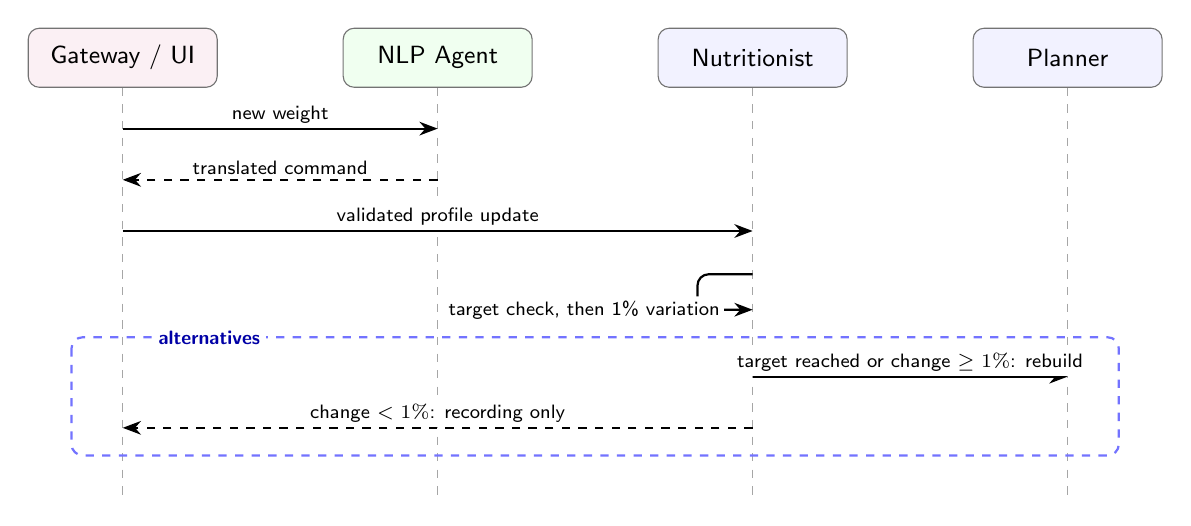
\begin{tikzpicture}[
    >=Stealth,
    actor/.style={rectangle, draw=black!55, rounded corners, fill=blue!5,
                  minimum width=2.4cm, minimum height=0.75cm, align=center,
                  font=\sffamily\small},
    message/.style={font=\sffamily\scriptsize, fill=white, inner sep=1.5pt}
]
\node[actor, fill=purple!6] (ui) at (0,0) {Gateway / UI};
\node[actor, fill=green!6] (nlp) at (4,0) {NLP Agent};
\node[actor] (nutri) at (8,0) {Nutritionist};
\node[actor] (planner) at (12,0) {Planner};
\foreach \x in {ui,nlp,nutri,planner} {
    \draw[dashed, black!35] (\x.south) -- ++(0,-5.2);
}
\draw[->, thick] (0,-0.9) -- node[message, above]{new weight} (4,-0.9);
\draw[->, thick, dashed] (4,-1.55) -- node[message, above]{translated command} (0,-1.55);
\draw[->, thick] (0,-2.2) -- node[message, above]{validated profile update} (8,-2.2);
\draw[->, thick, rounded corners] (8,-2.75) -- ++(-0.7,0) -- ++(0,-0.45) --
    node[message, left]{target check, then 1\% variation} (8,-3.2);
\draw[rounded corners, thick, dashed, blue!55]
    (-0.65,-3.55) rectangle (12.65,-5.05);
\node[font=\sffamily\scriptsize\bfseries, text=blue!65!black,
      fill=white, inner sep=2pt] at (1.1,-3.55) {alternatives};
\draw[->, thick] (8,-4.05) -- node[message, above]{target reached or change $\geq 1\%$: rebuild} (12,-4.05);
\draw[->, thick, dashed] (8,-4.7) -- node[message, above]{change $< 1\%$: recording only} (0,-4.7);
\end{tikzpicture}
\caption{UML diagram of the weight update}
\end{figure}

\subsection{Proactive monitoring, confirmation and different meal}

A \texttt{CyclicBehaviour} internal to the Nutritionist periodically injects a clock tick into
the BDI belief base. The AgentSpeak logic compares the current time with that of the previous
tick and requests confirmation
only for a slot whose time is crossed while the system is
running. The check is repeated at every tick for the entire duration of the
session. The user can confirm what was planned or indicate that
they consumed a different meal. In the latter case, the Cook estimates its
nutritional values and the Nutritionist possibly rebalances the subsequent meals of the
same day to compensate for any deviation from the plan.

\begin{figure}[H]
\centering
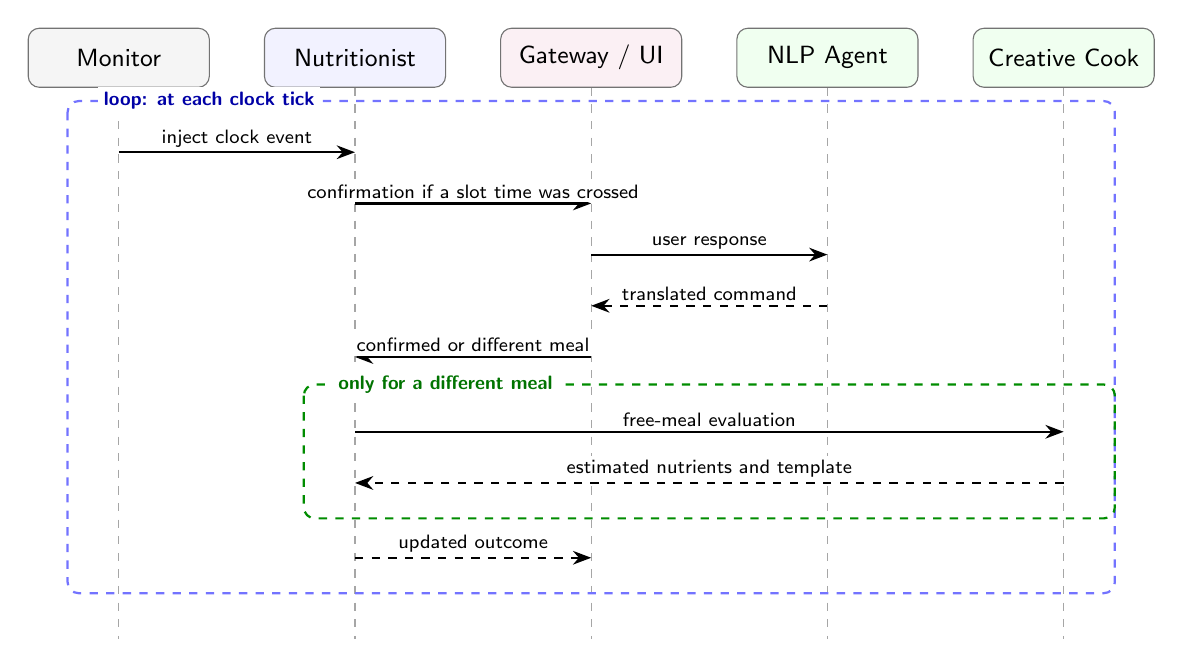
\begin{tikzpicture}[
    >=Stealth,
    actor/.style={rectangle, draw=black!55, rounded corners, fill=blue!5,
                  minimum width=2.3cm, minimum height=0.75cm, align=center,
                  font=\sffamily\small},
    message/.style={font=\sffamily\scriptsize, fill=white, inner sep=1.5pt}
]
\node[actor, fill=gray!8] (behav) at (0,0) {Monitor};
\node[actor] (nutri) at (3,0) {Nutritionist};
\node[actor, fill=purple!6] (ui) at (6,0) {Gateway / UI};
\node[actor, fill=green!6] (nlp) at (9,0) {NLP Agent};
\node[actor, fill=green!6] (cook) at (12,0) {Creative Cook};
\foreach \x in {behav,nutri,ui,nlp,cook} {
    \draw[dashed, black!35] (\x.south) -- ++(0,-7.0);
}
\draw[rounded corners, thick, dashed, blue!55]
    (-0.65,-0.55) rectangle (12.65,-6.8);
\node[font=\sffamily\scriptsize\bfseries, text=blue!65!black,
      fill=white, inner sep=2pt] at (1.15,-0.55) {loop: at each clock tick};
\draw[->, thick] (0,-1.2) -- node[message, above]{inject clock event} (3,-1.2);
\draw[->, thick] (3,-1.85) -- node[message, above]{confirmation if a slot time was crossed} (6,-1.85);
\draw[->, thick] (6,-2.5) -- node[message, above]{user response} (9,-2.5);
\draw[->, thick, dashed] (9,-3.15) -- node[message, above]{translated command} (6,-3.15);
\draw[->, thick] (6,-3.8) -- node[message, above]{confirmed or different meal} (3,-3.8);
\draw[rounded corners, thick, dashed, green!55!black]
    (2.35,-4.15) rectangle (12.65,-5.85);
\node[font=\sffamily\scriptsize\bfseries, text=green!45!black,
      fill=white, inner sep=2pt] at (4.15,-4.15) {only for a different meal};
\draw[->, thick] (3,-4.75) -- node[message, above]{free-meal evaluation} (12,-4.75);
\draw[->, thick, dashed] (12,-5.4) -- node[message, above]{estimated nutrients and template} (3,-5.4);
\draw[->, thick, dashed] (3,-6.35) -- node[message, above]{updated outcome} (6,-6.35);
\end{tikzpicture}
\caption{UML diagram of meal monitoring}
\end{figure}

\subsection{Replacement and rebalancing after a deviation}

When a different meal is recorded, the Creative Cook first estimates its nutritional values and
returns them to the Nutritionist. The Nutritionist compares the actual consumption with the daily
requirement and recalculates only the future meals of the same day. For each modifiable future slot,
the Planner, Chef and Creative Cook produce a strict replacement compatible with the diet, slot,
residual calorie target and scaled macronutrient target. This local procedure does not rerun the
global weekly variety and category-frequency search.
Compensation is limited by the availability of templates and realistic recipes, the system
does not force excessively reduced meals to recover the deviation.

\begin{figure}[H]
\centering
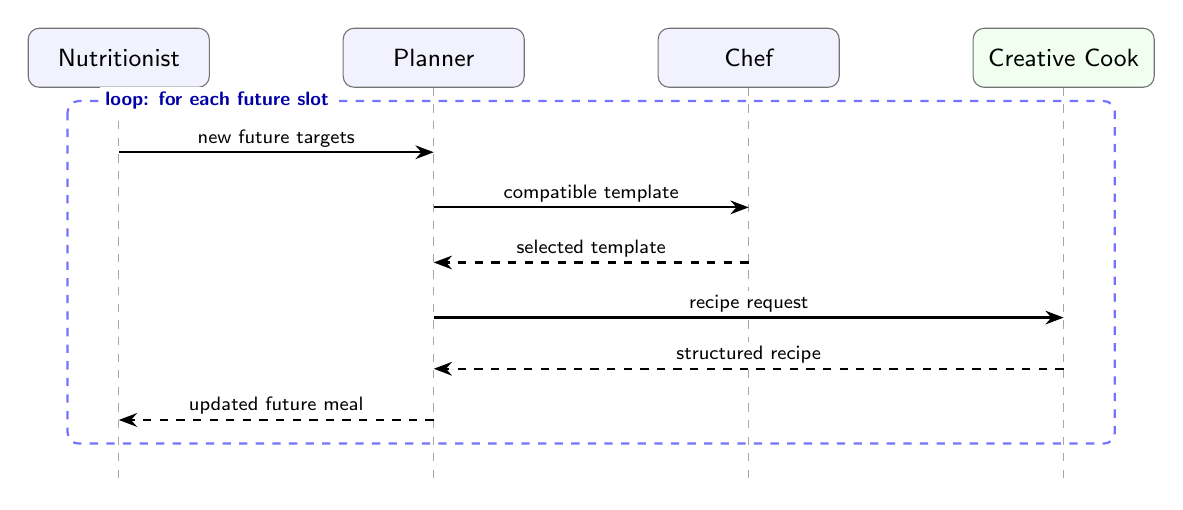
\begin{tikzpicture}[
    >=Stealth,
    actor/.style={rectangle, draw=black!55, rounded corners, fill=blue!5,
                  minimum width=2.3cm, minimum height=0.75cm, align=center,
                  font=\sffamily\small},
    message/.style={font=\sffamily\scriptsize, fill=white, inner sep=1.5pt}
]
\node[actor] (nutri) at (0,0) {Nutritionist};
\node[actor] (planner) at (4,0) {Planner};
\node[actor] (chef) at (8,0) {Chef};
\node[actor, fill=green!6] (cook) at (12,0) {Creative Cook};
\foreach \x in {nutri,planner,chef,cook} {
    \draw[dashed, black!35] (\x.south) -- ++(0,-5.0);
}
\draw[rounded corners, thick, dashed, blue!55]
    (-0.65,-0.55) rectangle (12.65,-4.9);
\node[font=\sffamily\scriptsize\bfseries, text=blue!65!black,
      fill=white, inner sep=2pt] at (1.25,-0.55) {loop: for each future slot};
\draw[->, thick] (0,-1.2) -- node[message, above]{new future targets} (4,-1.2);
\draw[->, thick] (4,-1.9) -- node[message, above]{compatible template} (8,-1.9);
\draw[->, thick, dashed] (8,-2.6) -- node[message, above]{selected template} (4,-2.6);
\draw[->, thick] (4,-3.3) -- node[message, above]{recipe request} (12,-3.3);
\draw[->, thick, dashed] (12,-3.95) -- node[message, above]{structured recipe} (4,-3.95);
\draw[->, thick, dashed] (4,-4.6) -- node[message, above]{updated future meal} (0,-4.6);
\end{tikzpicture}
\caption{UML diagram of rebalancing}
\end{figure}


\subsection{Plan consultation, recap and history}

The user can request the current plan, daily recap and meal or weight history.
The NLP translates the natural request and returns the command to the Gateway, which validates
and forwards it to the Planner or Nutritionist. The requested information is returned to the
Gateway and deterministically rendered in structured format without a second LLM translation.

\begin{figure}[H]
\centering
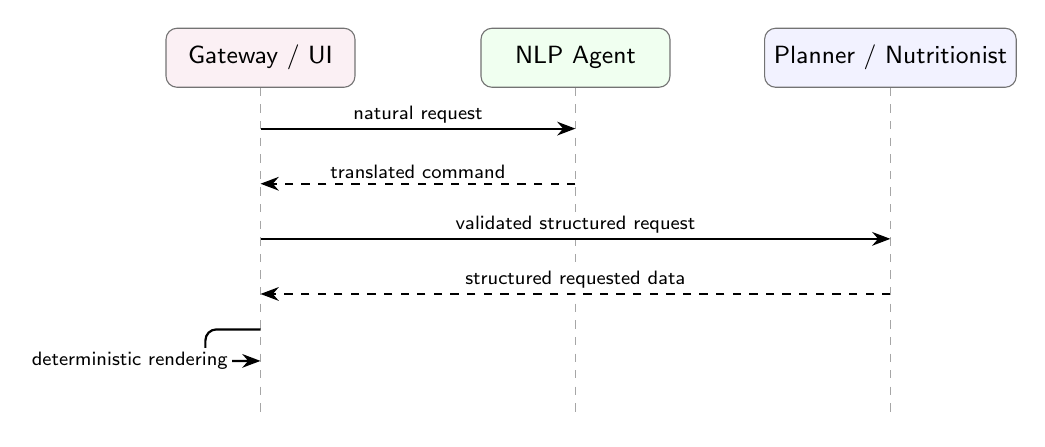
\begin{tikzpicture}[
    >=Stealth,
    actor/.style={rectangle, draw=black!55, rounded corners, fill=blue!5,
                  minimum width=2.4cm, minimum height=0.75cm, align=center,
                  font=\sffamily\small},
    message/.style={font=\sffamily\scriptsize, fill=white, inner sep=1.5pt}
]
\node[actor, fill=purple!6] (ui) at (0,0) {Gateway / UI};
\node[actor, fill=green!6] (nlp) at (4,0) {NLP Agent};
\node[actor] (domain) at (8,0) {Planner / Nutritionist};
\foreach \x in {ui,nlp,domain} {
    \draw[dashed, black!35] (\x.south) -- ++(0,-4.2);
}
\draw[->, thick] (0,-0.9) -- node[message, above]{natural request} (4,-0.9);
\draw[->, thick, dashed] (4,-1.6) -- node[message, above]{translated command} (0,-1.6);
\draw[->, thick] (0,-2.3) -- node[message, above]{validated structured request} (8,-2.3);
\draw[->, thick, dashed] (8,-3.0) -- node[message, above]{structured requested data} (0,-3.0);
\draw[->, thick, rounded corners] (0,-3.45) -- ++(-0.7,0) -- ++(0,-0.4) --
    node[message, left]{deterministic rendering} (0,-3.85);
\end{tikzpicture}
\caption{UML diagram of data consultation}
\end{figure}

\clearpage

\section{Demo}
\label{sec:demo}

\begin{figure}[H]
    \centering
    
\includegraphics[width=0.90\textwidth,height=0.90\textheight,keepaspectratio]{report/images/demo_onboarding.png}
    \caption{Onboarding and initial target calculation}
    \label{fig:demo-onboarding}
\end{figure}

\begin{figure}[H]
    \centering
    
\includegraphics[width=0.80\textwidth,height=0.50\textheight,keepaspectratio]{report/images/demo_monitoring.png}
    \caption{Monitoring and daily rebalancing}
    \label{fig:demo-monitoring}
\end{figure}

\begin{figure}[H]
    \centering
    
\includegraphics[width=0.70\textwidth,height=0.55\textheight,keepaspectratio]{report/images/demo_target_reached.png}
    \caption{Transition to maintenance after reaching the target}
    \label{fig:demo-target-reached}
\end{figure}

\begin{figure}[H]
    \centering
    
\includegraphics[width=0.90\textwidth,height=0.90\textheight,keepaspectratio]{report/images/demo_rebalancing_plan.png}
    \caption{Rebalancing of the weekly plan after a deviation}
    \label{fig:demo-rebalancing-plan}
\end{figure}

\begin{figure}[H]
    \centering
    
\includegraphics[width=0.99\textwidth,height=0.99\textheight,keepaspectratio]{report/images/demo_daily_plan.png}
    \caption{Consultation of the daily meal plan}
    \label{fig:demo-daily-plan}
\end{figure}

\begin{figure}[H]
    \centering
    
\includegraphics[width=0.60\textwidth,height=0.55\textheight,keepaspectratio]{report/images/demo_week_plan.png}
    \caption{Consultation of the weekly meal plan}
    \label{fig:demo-week-plan}
\end{figure}

\clearpage

\section{Limitations and open issues}
\label{sec:limitations}

\sloppy
\begin{itemize}
    \item \textbf{Translation from natural language}: the conversion of the user's requests into structured constraints is based on
    a finite set of manually defined templates and rules. The system can
    therefore prove fragile with respect to synonyms, unforeseen formulations,
    implicit constraints, or ambiguous requests.

    \item \textbf{Limited coverage of meal templates}: the templates used to build meals constitute a selected and manually encoded
    subset. Consequently, the variety of the generated plans
    depends on the coverage of the templates and does not include all the
    possible combinations of ingredients and recipes.

    \item \textbf{Simplification of the nutritional model}: the calculation of calories and macronutrients uses average values coming from the
    dataset and depends on the matching of ingredients and on the portions
    adopted. Furthermore, the generation of recipes through LLM can introduce
    ingredients or quantities not fully consistent with the selected template.

    \item \textbf{Heuristic definition of targets}: the nutritional targets are calculated by means of predefined formulas and coefficients
    applied uniformly to the different profiles. This approach
    simplifies the estimation, but does not model all the variables that influence 
    the actual individual requirement.

    \item \textbf{Local caloric rebalancing}: the rebalancing corrects the caloric deviation through a simplified modification
    of quantities. The procedure does not jointly optimize
    calories, macronutrients, food frequencies, variety, and compliance with
    constraints over the entire week.

    \item \textbf{Simplified management of allergens and dietary constraints}: allergens and preferences expressed in free text are translated into
    instructions for the Cook agent, but a structured representation
    of the relationships among ingredients, derivatives, food categories,
    and possible substitutions is not available. This limits the systematic verification of consistency
    between the declared constraints and the selected ingredients.
\end{itemize}
\fussy

\section{How to run the project}
\label{sec:execution}

From the repository root, it is advisable to create and activate a Python virtual environment,
then install the dependencies listed in \texttt{requirements.txt}:

\begin{lstlisting}
python -m venv .venv
.\.venv\Scripts\Activate.ps1
python -m pip install --upgrade pip
python -m pip install -r requirements.txt
\end{lstlisting}

Before startup, the two local configuration files must be prepared.
The repository includes example versions without credentials, which can
be copied with the following commands:

\begin{lstlisting}
Copy-Item config\.env.example config\.env
Copy-Item config\litellm_config.example.yaml `
    config\litellm_config.yaml
\end{lstlisting}

To start the entire system, the PowerShell script included in the
repository is recommended:

\begin{lstlisting}
.\scripts\run.ps1
\end{lstlisting}

\section{Use of Generative AI}

Generative AI tools were used as supporting instruments during the development of the project. 
Their use was limited to the following activities:

\begin{itemize}
    \item \textbf{Streamlit interface}: AI assistance was used during the implementation of the user interface, 
    allowing more development effort to be dedicated to the multi-agent architecture, 
    BDI reasoning and communication between agents.
    \item \textbf{Debugging support}: AI tools were occasionally used to investigate
    complex implementation issues. This was particularly useful when debugging
    AgentSpeak code, where untyped terms, complex predicates, and interactions
    between concurrent execution flows can make errors difficult to identify.
\end{itemize}


\makeatletter
\renewcommand{\@biblabel}[1]{\textbullet}
\makeatother
\begin{thebibliography}{9}
\raggedright
\setlength{\itemsep}{0.8em}
\setlength{\parsep}{0pt}

\bibitem{Mifflin1990}
M. D. Mifflin et al., ``A New Predictive Equation for Resting Energy
Expenditure in Healthy Individuals'', 1990. Article from which the
equation for estimating resting energy expenditure is taken.
\url{https://doi.org/10.1093/ajcn/51.2.241}

\bibitem{FSANZAFCDRelease3}
Food Standards Australia New Zealand, ``Australian Food Composition
Database -- Release 3'', 2025. Dataset from which the nutritional
values of the ingredients come.
\url{https://www.foodstandards.gov.au/science-data/food-nutrient-databases/afcd/data-files}

\bibitem{CDCBMI}
Centers for Disease Control and Prevention, ``Adult BMI Categories''.
Reference for the BMI thresholds used in determining
the initial goal.
\url{https://www.cdc.gov/bmi/adult-calculator/bmi-categories.html}

\end{thebibliography}

\end{document}
